% Chapter 3

\chapter{Methods and Reflexivity} % Chapter 3 title

\label{Chapter3} % For referencing the chapter elsewhere, use \ref{Chapter3} 

%------------------------------------------------------------------

 When I began this research in 2017, I purposed to engage Neonatal Intensive Care Unit (NICU) staff and mothers of premature infants in the design process of a possible NICU communication intervention that would enhance Mothers-staff communication. We focused on  unveiling the impact of the design process on the participants by carefully monitoring the effects of the research methods applied in the study. This being a sensitive study that engaged participants who have gone through emotional lifetime in the NICU, our methodological choice focused on empowering the participants and encourage relationship between the multiple stakeholders to ensure that they work together in identifying possible communication solution in the NICU. 
 
 As the researcher, the NICU was an unfamiliar environment and I was aware the process of unveiling some of the idiosyncrasies of participants and neonatal unit circumstances would not be linear. NICU is an emotionally charged environment and this inevitably implicated a range of potential contributory causal factors, multiple perspectives and interpretations. To familiarize with this environment, I opted to work as a volunteer in the neonatal unit where I helped the nurses to cup feed and clean the infants. I also supported the mothers in the unit every time they needed my assistance.  The interactions with nurses and mothers helped me to understand the NICU workflow and the challenges they face in the NICU as they collaborate in infant care.
 
 The main objective of this research was and still is to explore and identify appropriate co-design methods that would fully engage NICU stakeholders in a sensitive design process of a possible NICU communication intervention. In preparation of this process, I selected a list of methodological approaches which would enhance participants' empathy throughout the design process to ensure that the risk of false starts were mitigated. Despite being aware of possibility of methodological pitfalls, I still fell into some. To bypass these pitfalls, I adopted iterative methods that helped me to identify and analyse the strength and shortcoming of each method. Eventually each method was modified accordingly to ensure it helped participants to untap their design skills and empower them to use their knowledge and experience to define the design process. In so doing, my role as HCI researcher was to empower the stakeholders to fully engage not just in design, but in clear articulation of their technology desires. I focused on facilitating the co-creation process instead of getting too bogged down in 'helping" stakeholders in design process. This adheres to \textcite{Rogers2013} approach which demonstrated that when participants are empowered, they become better equipped with technological skills which enable them to innovate for themselves.
 

\section{Identity and Self Positioning Within the research}
In this section, I discuss my methodological choices with respect to my positioning in this research. Given my research focused on exploring the appropriate methods that could fully engage both parents and NICU staff in the co-design process, I will use Interpretive Phenomenological Approach (IPA), which is a qualitative method that focuses on seeking out the meanings of individual experiences and how these meanings influence the choices made in a research \citep{peat2019, Smith2007}. IPA was originally developed as a method to undertake experiential research in psychology and it has gradually gained recognition in other fields to explain the researcher's understanding and interpretation of research topics through a process of in depth
reflective inquiry \citep{Smith1996}. In this study, I used IPA to understand the NICU context and explain how my ongoing methodological choices influenced participants engagement in the design process by providing my insights as I explored multiple realities through a reflexive process to interpret my experiences during the design process. In regard to this, I choose to write this document in the first person. However, occasionally  I will use 'we' to acknowledge instances where my colleagues contributed to this study.

\subsection{Researcher with No Neonatal Unit Experience}
Before I started doing this research in 2017, I had prior experience of working with mothers in developing world context. However, I had not worked in neonatal unit environment. Being a woman of child bearing age, my initial NICU visits were disturbing as well as intriguing. The environment was filled with an emotional cloud and I was compelled to immerse in this research and use my previous design and computer science skills to explore possible solutions that could improve the stressful experiences in the NICU. 

Unlike in my career practice where I utilized random ethnography (due to time limitation) to understand end users, in this case, I had to conduct a longitudinal study to understand the NICU ecosystem. Since I was going to involve participants in their social setting, I needed to take a reflective approach to thinking about the methodology and methods selection and their effect on participants engagement in the design process. Eventually, I opted to use co-design approach which is a Human Computer Interaction (HCI) method that is advocated especially when developing new solutions for marginalised and vulnerable people in developing countries \cite {Sharma2008}. This approach share the view that every participant is an expert in how they live their lives and that design ideas arise in collaboration with participants from diverse backgrounds \citep{Sanoff2016}. We thought this was the appropriate methodological approach because it would help us understand NICU experience from different perspective and  focused on empowering participants by allowing them to partake and lead in the design process.

To familiarize with NICU environment, I volunteered to work in the unit. I registered with the benevolence office at the hospital and offered to assist with the duties at the NICU.  My role was to help the nurses to clean and feed the infants whose health was stable and awaiting to be discharged. In addition, I supported mothers in the unit by helping them to fetch infants clothes from the drawer and labeled expressed milk from the fridge. Working in the unit at the initial stage of this study gave me an opportunity to observe and understand the NICU workflow, interaction between staff and mothers and the communication gaps that existed in the unit. In addition, I was able to learn the different cultural backgrounds of both the parents and NICU staff and their effect of NICU communication. With the NICU ecosystem in my mind, I was able to vaguely comprehend the communication challenges in the unit. This prompted me to indulge in several activities in the unit to support nurses who juggled between several roles due to staff shortage, as well as mothers who were adjusting to NICU environment. These activities are discussed in detail with respect to needs assessment process in section \ref{Activities}

My position as a volunteer worker in the NICU provided an opportunity for me to interact with nurses and mothers which eventually led in building trust and working relationships. These interactions provided an opportunity for mutual education process. Involuntarily, nurses and mothers shared their challenges in the NICU and they upheld my research ideas which focused on alleviating the communication challenges they were facing in the unit. Eventually, this eased my recruitment process because most NICU staff were aware of my research objective and they were willing to engage in the design process hoping that the overall outcome will support and improve their communication role in the unit. 

Being a female researcher, made it easy for participants to interact with me throughout the study. However, initially, nurses in other sections in the unit (other than the the one I allocated to volunteer) assumed I was supervising them.  Despite being introduced as a researcher by the  unit supervisor, they keenly conducted their day to day role as they observed my reaction to their actions. This affected my data collection process and I had to inform them that I was not there to report on them but to work closely with them to identify common NICU communication challenges and possible solution. This created a calm working environment in the unit helping me to identify the real communication gaps.

On the other hand, mothers thought I was a staff in the NICU and they approach me to help them access medical information. Unfortunately, I was not in a position to share the information. Instead, I acted as a mediator between parents and NICU staff. I would relay the information to the NICU staff who in return  provided parents with the medical information requested. However, the mediator 'role' did not go well when the NICU staff forgot to call or share information with the mothers. Mothers called me frequently and I had to visit the unit to remind the staff to call the mothers. These experiences gave me additional insight on the specific information needed by mothers of premature infants.

\section {Co-design Activities}
In this section I discuss the  co-design phases in this study and the methods and approaches that underpinned this work. We modified and localised these methods to adhere to the culture, NICU experience and technical exposure of the participants of this research to encourage them to fully engage in the design process. Table~\ref{Table: 28 months study} and figure~\ref{fig:timeline} provide an overview and timeline of each phase. This research was conducted over a period of 28 months.

\subsection{Co-design Approach}
We employed co-design approach, engaging participants (in this case NICU staff and mothers) as active research participants throughout the design process. Co-design is a creative practice that allows participants to engage in formulation of a possible solution throughout the design process to ensure the results meet their needs and are usable \citep{Sanders2008a, Nilsson2016}. Co-design, acknowledges that the ability to design is inmately human  and everyone can imagine, define and plan the transformation of their current scenario to ensure that the outcome meets their needs and expectations~\citep{Saunder2011, SarmientoPelayo2015}. Unlike the traditional focus of the practice of design where users are only engaged during data collection and evaluation process, co-design is practiced using a \textit{design-with} mindset that allows the designers or design researchers to use the ideas generated by others as sources of inspiration and innovation.

Within health care, co-design has been mainly employed as a way of designing better experiences for patients, carers, and staff~\citep{Piper2018, Timmerman2016, Ward2018}. Various researchers have emphasized the the importance of  using co-design approach in health system design process \citep{Piper2018, Timmerman2016, Birnbaum2016, Wolstenholme2017, Robert2015}. This is due to the fact that co-design encourages users' engagement through participatory or empathic methods \citep{Piper2018}. Participatory methods embraces democracy during the design process thus enabling all participants to play an active and influential part in decisions which affect their lives \citep{Wadley2016, Hussain2012}.  On the other hand, empathic methods help the designer/researcher to deepen the understanding of the end user, in a way that intangible concepts such as feelings, emotions, aspirations and fears provide the designer/researcher with clues of how stakeholders see, understand and interact  with the world around them \citep{SarmientoPelayo2015, Schneider2018a}. As a result, these clues inspire design of a product with a better functional balance, which, in turn, provide pleasurable experiences of use to the end-users.

Based on the aformentioned aspects, I chose to employ co-design strategy in the NICU environment and focus on using it as empowerment tool for the  participants. According to \textcite{Schneider2018}, co-design advocates design and developing of tools that people can use actively and creatively thus empowering them. This being under-researched environment with limited previous literature providing design recommendations, I chose to go beyond consultation and testing of already developed sketches or interventions. Rather, I sought to engage participants as co-designers to understand their needs and design a solution with them to meet those needs. This active participation of participants follows human-centered design principles that tend to focus on needs, contexts, behaviors, and emotions of the people that the solutions will serve \citep{Blandford2018, Buchanan2001}. Consequently, this process could provide a sense of ownership among the participants because it enables them to tailor the intervention to their specific cultural needs and contexts. In addition, \textcite{Verbiest2018} argues that this approach often contributes to better uptake of health care system.  In the remainder of this chapter I describe the methods and approaches that underpinned this work. I reflect on the challenges I faced and how they influenced my methods selection and interactions with the participants.

\subsection{ Research Phases and Activities} \label{Activities}
This study comprises of six phases which were conducted in a span of 28 months. In the first phase (reported in details in \ref{Chapter4}) that ran for six months, we engaged mothers of preterm infants---who had been discharged from the hospital for at least two months---and NICU staff to assess the communication needs and challenges in the NICU. I used observation and interviews to understand the NICU environment activities and challenges in depth. The observations were conducted in two parts. In the first part, I worked closely with NICU staff to understand the unit's workflow and interactions. In the second part, I visited the unit both during the day and night to gain insights of the unit's activities from multiple perspectives. This being a new and sensitive research environment, observation gave me access to the explicit and observable aspect of parents and NICU staff lives. Although initially I was scared of the environment, I was able to understand the NICU in depth before engaging with participants in interview sessions. The interviews feedback reinforced and expanded on the observation sessions findings. I used \textit{context mapping} \citep{Offermans2014} technique to understand participants experiences and aspiration by eliciting deeper needs of every participating participants. Through this, I identified participants' fears, emotions and aspirations which instigated the need for modification/alteration of research design and methods in subsequent data collection phases. I did this to ensure the study adhered to design ethics without inflicting pain or stress to the participants. The data collected in this phase was thematically analysed using nVivo software. The identified themes were used as the input information for subsequent phases.

The second and third phases that ran for seven months, were designated for design ideas generation and exploration process. During this period, I engaged mothers, doctors and nurses to identify and define the communication problems in the NICU and possible interventions that could be adopted to solve the problems identified in the first phase. I employed \textcite{Marsden2008} empowered design  that recognises that when empowered, people with limited exposure to technology are able capable of moulding technology solutions to meet their own needs. To achieve this objective, we chose to use focus groups, brainstorming and sketching methods to facilitate collaboration and creativity among the participants. This was achieved by setting the phases in iterative cycles of problem setting and solution finding. This approach encouraged participants to use their NICU experiences to model a solution that could suit their own context. However, there was power inequalities during these sessions which hindered some participants from engaging in the design ideas generation. We opted to include other methods such as \textit{role playing}~\citep{Lawson2016}, \textit{card sorting}~\citep{Nakarada-Kordic2017}, \textit{scenario}~\citep{Nardi2007} together with generative techniques such as \textit{context mapping}~\citep{Offermans2014} which enabled shy participants to engage in a constructive design discussion. With ethics considerations in mind, I decided to pair methods and explore their effects on information sharing process and also to allow the methods to reinforce and complement each other enabling triangulation of data. 

For instance, I paired role playing and participants' real life scenario to built user empathy which consequently gave me new insights which I could not understand during the focus group sessions. Also, use of card sorting during the brainstorming sessions enabled shy participants to articulate their ideas and structure them in a manner that makes sense to them. However having each group of stakeholders in their separate groups before merging them in one multistakeholders (nurses, doctors and mothers) group limited the collaboration which was essential to ensure that the final tool incorporated all their design decision. Furthermore, this approach neither encouraged mutual learning among participants nor eliminated power inequality in decision making. Instead, mothers agreed with all the decisions made by NICU staff even though they did not follow mothers' idiosyncratic interests. In response to these findings, I decided to change the strategy and have all stakeholders in a joined brainstorming session in subsequent sessions.

In phase four (14-22 months), I engaged mothers and NICU staff to collaborate in sketching the final prototype of the proposed solution and explore appropriate ways of representing and visualizing the information suggested in previous phases. Although I purposed to work with mothers whose children had been discharged from the hospital, we encountered low turn out of mothers which prompted us to navigate the approved theoretical ethics and work with mothers of infants in the NICU with stable health and awaiting to be discharged. To ensure that the study had no negative effect on these mothers, we focused on fostering mutual learning between mothers and NICU staff to enhance relationship and empower them through NICU information sharing. To achieve this objective we used focus group and interactive prototyping sessions. Unlike in the previous phase where we had separate sessions with different stakeholders, we choose to have one focus group with multiple stakeholders to foster relationship and built trust among them. During the focus group session we opted to use \textit{series of unanswered questions} and asked participants to use their NICU experiences to simplify the information suggested in previous phase. We later engage them in a collaborative prototyping session which aimed at visualizing the suggested information in a simple format that mothers could understand. We used generative techniques such as \textit{sketching}, \textit{card sorting} and \textit{emoticons} to encourage collaboration among multiple stakeholder with no prior design skills.

This approach encouraged the participants to share their NICU experiences and engage in exploring the most viable communication intervention in NICU context. It also supported mutual learning and empathy building among participants. Relationships and trust among participants were boosted during the discussion, fostering creativity and ideas sharing. This was achieved as a result of design activities being completely led by the participants. The research assistance and I took a step back in acceptance that the participants had a vast NICU experience warranting them all the privileges in shaping the design ideas. Our role was only to support the participants design activities as we visualize their ideas on a workflow. We also facilitated the collaborative sketching sessions ensuring that participants had access to all the materials required to actualize their ideas. 

This approach influenced changes in design and workflows developed in previous phases. Participants devised best ways of accessing and sharing information in a resource constrained environment in manner that fits within the stressful NICU context (See chapter \ref{Chapter5}). I analysed the data collected and used the final paper prototype to develop the proposed mobile application in three different languages: English, IsiKhosa and Afrikaans. We later tested the applications before deploying them at the hospital for the mothers to use them while their infants are admitted in the unit.

In month 22-25 (eight months) we deployed the intervention in the NICU and evaluated its effect on  the communication between mothers and the NICU staff. We also focused to investigating whether the information provided helped to alleviate the stress related to premature births among mothers. We worked in the unit for two weeks as we trained, monitored and supported mothers and NICU staff as they interacted with the application. We used observation, cognitive walkthrough and follow up interviews to evaluate participants interactions and experiences with the deployed intervention. We  further logged usage of the tool and conducted an analysis (reported in details in \ref{Chapter6}).

For three months (26-28 month) we trained the nurses and NICU clerks on how to manage the tool and later launched the communication tool at the hospital for continuous monitoring. I focused on monitoring and studying the use of Preemiecare system. This involved further analysis of the system usage logs. We followed up the analysis with brainstorming session with the stakeholders to understand the positive and negative outcome of the project and to understand strategies of improving the usability and positive effects of the intervention.

The approach we chose demonstrated the importance of using participants' real life experiences to mould the design of a possible intervention that could address the communication challenges they face in the NICU. We used different methods pairing them to ensure mutual learning and relationships between multiple stakeholders are enhanced during the  design process. We describe these results in detail in the three chapters that follow.

\begin{table}[thb]
    \centering
    \begin{tabular}{|p{4.6cm}|c|c|p{4.5cm}|}
        \hline
        \textbf{Phase}  & \textbf{Duration} & \textbf{Participants} & \textbf{Methods}  \\ \hline
        Needs Assessment and    &     6 months          & 15 mothers   & Observation\\
       Problem Identification &     & 15 NICU Staff & Semi-structured Interviews \\ \hline
        Ideas Generation  and & 7 months  & 8 mothers         &    Focus Groups     \\
        Exploration &    & 10 NICU Staff & Brainstorming \\
         &     &   & Role playing \\
            &     &   & Scenarios \\\hline
            Prototyping &  8 months & 6 mothers & Focus Groups \\
            &  & 6 NICU Staff & Sketching \\
            & & & Series of unanswered questions \\
               & & & Card Sorting \\
                  & & & Emoticons \\
                   & & & System Coding \\
                  \hline
                    System Deployment & 3 months &25 mothers & Observation \\
                       &  & 10 NICU staff& Interviews \\
                          & & & System Logs analysis \\
                          \hline
                            Handover & 3 months & 4 NICU staff& Staff Training \\
                               & & & Brainstorming \\
                                & & & System Logs analysis \\
                            \hline
    \end{tabular}
    \caption{Overview of methods used, duration, and the number of participants involved in the 28 months study.}
    \label{Table: 28 months study}
\end{table}

\begin{figure}[htp]
    \centering
    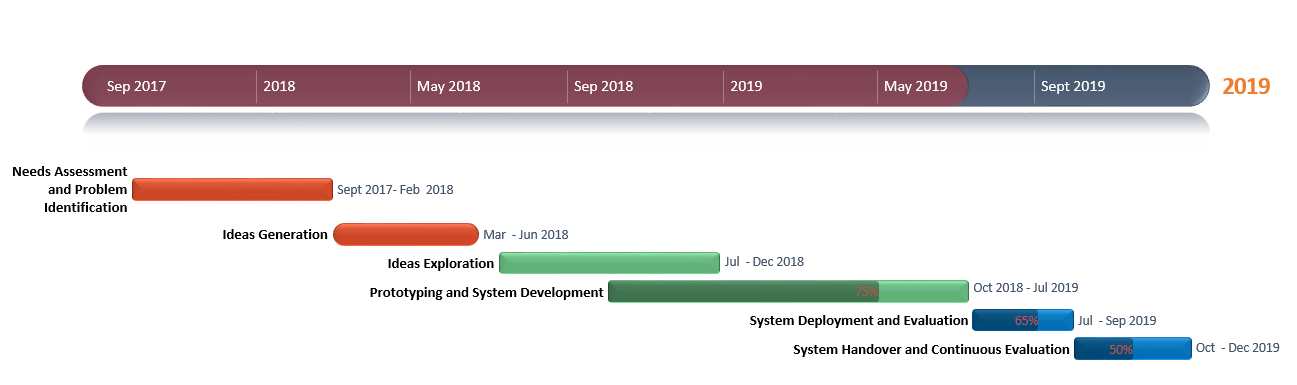
\includegraphics[width=17cm, height=10cm]{Figures/save.PNG}
    \caption{Overview of the 28-Month Study.}
    \label{fig:timeline}
    \end{figure}

 \section{Methodological Challenges in NICU Context}
 Throughout the co-design process, we encountered four co-design dynamics namely 1. power dynamic 2. shyness and fear 3. conflicts and disagreements and 4. group thinking (discussed in detail in the next three chapters) which affected the co-design process. To mitigate these dynamics and foster relationship between participants, we opted to use generative techniques such as incomplete sentences, emoticons, contextual map, role-playing, braindumping and scenarios to encourage all participants to voice their design decisions and engage in the discussion. 
 
 Although the co-design dynamics were not eliminated immediately, the use of mediated interaction approach through the generative design techniques helped the participants to gradually collaborate and work towards the common goal which was to design a tool that could enhance NICU communication. During the design process, I was able to build a deeper and more longitudinal understanding of the methodological considerations especially while working with multiple stakeholders in a sensitive NICU context. I realized that as a researcher, I need to have a list of several participatory methods---which I refer as "\textbf{basket of methods}"---that need to be modified, localized and paired before use to explore and achieve desirable outcomes. Methods  alteration and localization is necessary in sensitive context to ensure they align with the participant's cultural norms and environment.
 
 As a researcher undertaking qualitative research on sensitive topics, I learned the importance of assessing the impact of the research on the participants and myself. In this study, I faced many challenges including developing friendships, working relationships, emotional and physical safety, and conflict over roles. Most of the time, I neglected the negative effect that the study had on me and focused on ensuring that my participants were safe. I understood I was entering the lives of my participants at a time of stress and I focused on reducing any chance that could exacerbate their level of stress. However, this process made me feel uneasy about the level of disclosure during the interview sessions. At some instance, I got emotional and I had to divert the discussion to hide my emotions from the participants. This provided an opportunity for mothers to ask me unexpected questions about my personal life. Although I was not prepared for the self-disclosure, I felt like this opportunity was an important part of rapport-building process and I opted to use it to put myself on a level playing field with the participants.
 
  In addition, as a Kenyan computer scientist conducting research in South Africa, I encountered language barrier which hindered my interaction with participants during the co-design process. Some participants were hesitant to open up to me in recognition that my accent was different from the common South Africa accents. This was even worse when I arranged for follow up meetings in mothers' homes. They did not invite me to their homes due to security issues (i.e if a foreigner or visitor goes to their home, they become a target to the community gangs) but instead, they suggested we meet in public hospitals or police station. To build trust and enhance engagement in this study, I explicitly discuss the benefit of the research with participants (mothers and NICU staff) before delving into the data collection process. In some instance, I had to modify the research design to fit into the culture and beliefs of the participants.
 
\subsection{Working With Multiple Stakeholders}
Co-design is recognized as a methodology that supports inclusive problem solving and solutions finding~\citep{Jones2008b}. It places multiple stakeholders with disparate real life experiences and skills/knowledge to spend quality time mapping their journeys, identifying problems and developing possible solution that could mitigate the identified obstacles. However, this process is complex among multiple stakeholders because it increases the diversification through the the broadness of information, knowledge and suggestions of possible solutions. In this study, these differences led to co-design dynamics such as power dynamic, conflicts and group thinking which hindered collaboration. The hierarchical infant care structure in the NICU made the doctors and nurses to dominate the design dialogue thus limiting the mothers from sharing their design views. 

Attempt to counter these co-design dynamics and build relationship and trust among stakeholders demanded the use creative design approaches such as modification of methods, pairing of several methods etc. to encourage new ways of thinking that fostered collaboration among stakeholders. My methodological choices drew from literature in maternal and child care health, human-computer interaction for Development (HCI4D), psychology and Information Communication and Technology for Development (ICT4D). Although my experience and knowledge in health and psychology is limited, I occasionally use the basic knowledge gained through the online courses that I pursued to identify potential problems that commonly arise with various methods in these fields. 

Methodological considerations thus made from these multidisciplinary fields made my solution exploration approach more of a "trial and error". This approach although challenging, helped me learn that methodological solution in such sensitive interdisciplinary studies are not achieved immediately as one would expect. Instead, it takes time and effort to understand the environment and the people to ensure that the co-design process empowered the stakeholders to articulate the needs that they want to jointly meet with the researchers/designers.

For instance, I spoke to different groups of stakeholders (nurses, doctors, mothers, NICU supervisors) who had different needs with some of them not aligned with our research objectives. They all wanted the study to focus on their group specific communication needs so as to make their infant care role easy. Holding separate stakeholders focus groups, made me become aware of the broad and specific interest and goals of each group.  However, it was impossible to meet "everyone's" needs and requirements. Rather, I decided to have joint focus group with multiple stakeholders encouraging them to negotiate their disparate requirements. Based on their different NICU experiences, they were able to interact and cooperate constructively with each other in such a way that their different goals were addressed simultaneously.

\subsection{Understanding the Self in Conflict and Emotional Situations}
There were several instances when conflicts and disagreement arose during the design process. This depicted the hierarchical working relationship in the unit that hindered effective communication. As a researcher, this created an awkward design environment which I had no experience on. Hence, I opted not to interject the discussion but instead facilitate the sessions to ensure the discussion led to a constructive argument that would help participants to articulate their needs and technology desires.~\textcite{Rogers2013} insist that HCI researchers should focus on facilitating the design process and refrain from helping or engaging in the design process a discourse they refer to rhetoric of engagement. To adhere to this discourse, I chose to remain as researcher and put my effort in exploring different methods to encourage collaboration and enable participants to reach to a consensus. This helped me to understand the different perspective of participants, enabling me to see design ideas through their lens and learn why they are pushing back on other participants' ideas. 

\subsection{Emotional Effects on the Researcher} 
In the initial stages of this research, I experienced emotional difficulties as I conducted interviews to understand the NICU experiences and challenges  from the participants. The life experiences shared by participants---especially the mothers; were sad and had emotional toll on both the participants and myself. In such instances,  I evaded these emotional instances by diverting the discussion to a general talk such as baby's feeds and development to ensure that the participants and myself were emotionally stable by the end of the session. Also, I chose to play around with the children using the colourful audio picture books given to the mothers as a honorarium. Although these were temporary solutions, the interjection positively changed mothers' mood as they watched their children enjoy playing with the audio picture book. 

In cases where mothers needed further counseling services, I made arrangements with the nurses in the hospital who offered the needed support.  These emotional scenarios helped me to learn the importance of having counseling knowledge or skills as a researcher especially while engaging with vulnerable participants. In addition, I learned that researchers should have a flexible research plan that allows them to navigate ethics in cases where ethics in practice reveal new ethical dimensions. These ethics challenges in co-design research provides opportunities for consideration and improvement especially in HCI research ethics review processes.

\subsection{Considering Self-Care in Emotionally Demanding Research}
Prior to this study, I pursued online courses to help me to understand the sensitivity of this research and identify participants in case they were emotionally disturbed. Despite this preparation, I did not have access to information that could support me handle emotions as a researcher. As a result, I found myself engulfed with emotions as I engaged with participants during the problem identification phase. I did not pay attention to my emotions but instead focused on ensuring that participants emotional status was stable. I was not doing justice to myself and I would advise researchers conducting research in such sensitive settings to consider their physical and mental well being as they aspire to ensure that the research does not harm the participants. 
 
This consideration should be given a thought at the inception of the research. I learned the importance of providing practical suggestions while seeking ethical approval from Institutional Review  Board (IRB). I should have ensured that the ethics application protected both the participants and myself as I focus on achieving the stipulated  ethics. Instead, I upheld a naïve view of what such sensitive research studies and participants' collaborations require in terms of time and resources. As a result, planning and adhering to the approved  research ethics was challenging and I had to navigate the ethics as I focus on the  safety of the participants in order to achieve the research objectives.

\subsection{Methodological Consideration in Emotionally Charged Environment}
Base on the knowledge I acquired from the online courses, I was able to select methods that considered the sensitivity of the topic ensuring that the psychological aspect of the participants was protected. This was achieved by encouraging mutual learning concept during the design process to ensure the participants---especially the mothers, benefited from the exchange of the information. In addition, I learned the importance of focusing on taking precautions to reduce the effects of study on the participants by adopting suitable strategies such as duration and intensity of interviews, choice of question etc. Following these reflections, I recommend HCI researchers to focus on using research methods as a means to establish a relation of trust, because proximity and familiarity with the participants facilitates mutual knowledge. This is the only way to get oneself accepted thanks to a gradual entry that helps to minimise the social distance.

Through out the study, I sought to understand the impact and effect of the methodological decision I made as a researcher. Indeed the process has numerous pitfall which we drew lessons from. I learned that as a researcher engaging with participants in co-design to create supportive technological interventions, I need to be mindful of what I can offer ensuring that I do not impose my needs on them. Instead, I should leave the appropriation and innovation of technologies to the users of the technologies. \textcite{Taylor2011} findings reinforce my sentiment by arguing that HCI researchers should not frame and solve issues based on their theories rather they should provide practical tools that support engagement and new ways of learning to the participants. In that respect, we put our focus on methods that would enhance participants relationship ensuring that the hierarchical structure in the unit did not hinder some participants from voicing their design ideas. This was achieved by using paired methods in phased co-design approach. 

\section{Chapter Summary}





% This just dumps some pseudolatin in so you can see some text in place.
%\blindtext
